\documentclass[12pt, oneside]{book}

% toto som navysil!

\usepackage[a4paper,top=3cm,bottom=3.5cm,left=3cm,right=3cm]{geometry}
%\usepackage[a4paper,top=2.5cm,bottom=2.5cm,left=3.5cm,right=2cm]{geometry}

\usepackage[utf8]{inputenc}
\usepackage[T1]{fontenc}
\usepackage{graphicx}
\usepackage{url}
\usepackage{float}
\usepackage{listings}
\usepackage[english]{babel} % vypnite pre prace v anglictine
\linespread{1.25} % hodnota 1.25 by mala zodpovedat 1.5 riadkovaniu
\usepackage{xcolor}
\usepackage{textcomp}

\lstset{frame=tb,
  language=PHP,
  aboveskip=3mm,
  belowskip=3mm,
  showstringspaces=false,
  columns=flexible,
  basicstyle={\small\ttfamily},
  numbers=none,
  numberstyle=\tiny\color{gray},
  keywordstyle=\color{blue},
  commentstyle=\color{green},
  stringstyle=\color{blue},
  basicstyle=\tiny,
  breaklines=true,
  breakatwhitespace=true,
  tabsize=3,
}


% -------------------
% --- Definicia zakladnych pojmov
% --- Vyplnte podla vasho zadania
% -------------------
\def\mfrok{2016}
\def\mfnazov{Assignments Workflow in Learning Management System}
\def\mftyp{Diploma thesis}
\def\mfautor{Bc. Tomáš Trungel}
\def\mfskolitel{RNDr. Martin Homola, PhD.}

%ak mate konzultanta, odkomentujte aj jeho meno na titulnom liste
\def\mfkonzultant{doc. RNDr. Zuzana Kubincová, PhD.}  

\def\mfmiesto{Bratislava, \mfrok}

%aj cislo odboru je povinne a je podla studijneho odboru autora prace
\def\mfodbor{2511 Applied Informatics} 
\def\program{ Applied Informatics }
\def\mfpracovisko{ Department of Applied Informatics }

\begin{document}     

% -------------------
% --- Obalka ------
% -------------------
\thispagestyle{empty}

\begin{center}
\sc\large
Comenius University in Bratislava\\
Faculty of mathematics, physics and informatics

\vfill

{\LARGE\mfnazov}\\
\mftyp
\end{center}

\vfill

{\sc\large 
\noindent \mfrok\\
\mfautor
}

\eject % EOP i
% --- koniec obalky ----

% -------------------
% --- Titulný list
% -------------------

\thispagestyle{empty}
\noindent

\begin{center}
\sc  
\large
Comenius University in Bratislava\\
Faculty of mathematics, physics and informatics

\vfill

{\LARGE\mfnazov}\\
\mftyp
\end{center}

\vfill

\noindent
\begin{tabular}{ll}
Study programme: & \program \\
Field of study: & \mfodbor \\
Department: & \mfpracovisko \\
Supervisor: & \mfskolitel \\
Consultant: & \mfkonzultant \\
\end{tabular}

\vfill


\noindent \mfmiesto\\
\mfautor

\eject % EOP i


% --- Koniec titulnej strany


% -------------------
% --- Zadanie z AIS
% -------------------
% v tlačenej verzii s podpismi zainteresovaných osôb.
% v elektronickej verzii sa zverejňuje zadanie bez podpisov

\newpage 
\thispagestyle{empty}
\hspace{-2cm}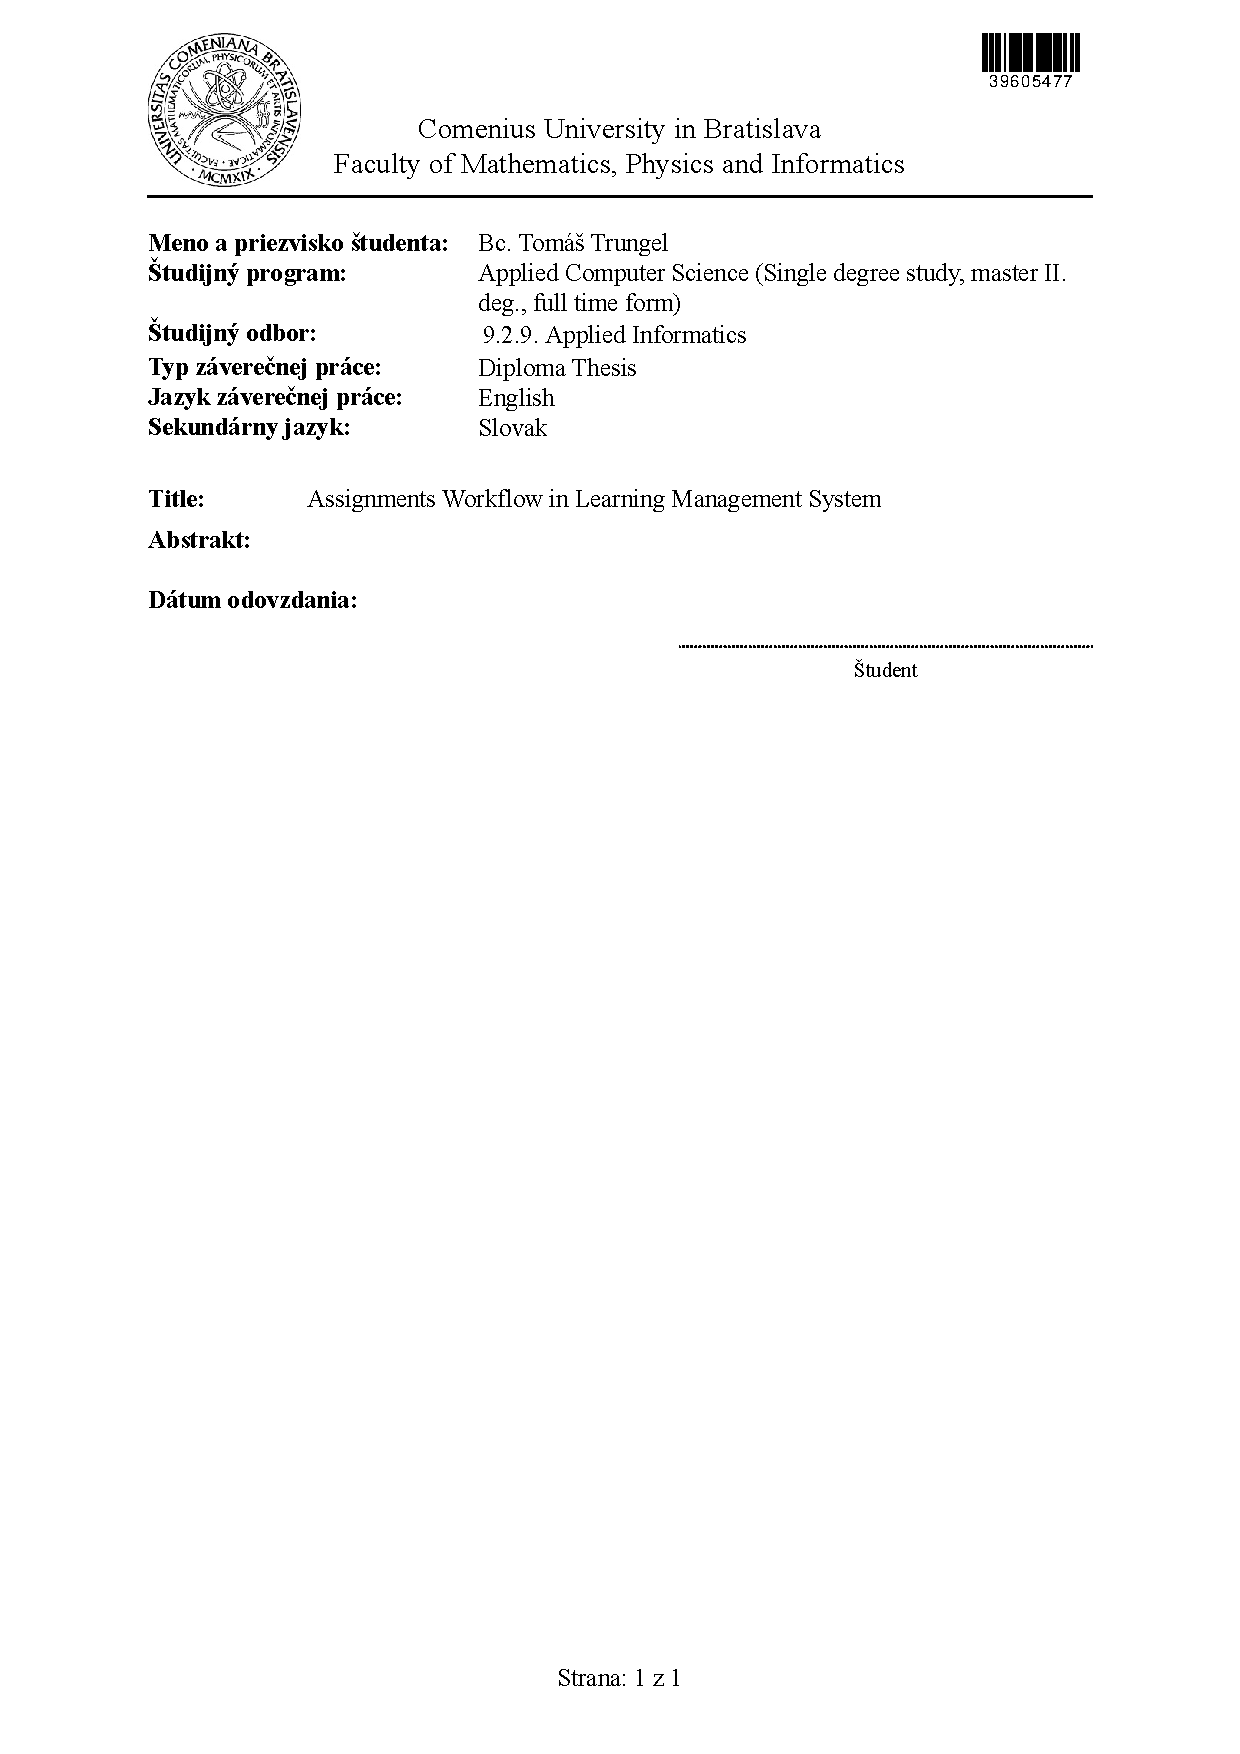
\includegraphics[width=1.1\textwidth]{images/zadanie}

% --- Koniec zadania

% --- Copyright
\newpage

\noindent
\begin{minipage}{0.25\textwidth}~\end{minipage}
\begin{minipage}{0.68\textwidth}
By this I declare that I wrote this master thesis by myself, only with the help of the referenced literature, under the careful supervision of my thesis advisor.
\bigskip\bigskip

\hfill\hbox to 6cm{\dotfill}
\end{minipage}
\vfill\eject % EOP iii
~\vfill\eject % EOP iv


% ---- End copyright

\frontmatter

% -------------------
%   Poďakovanie - nepovinné
% -------------------
\setcounter{page}{3}
\newpage 

\begin{minipage}{0.25\textwidth}~\end{minipage}
\begin{minipage}{0.68\textwidth}
{\bf Acknowledgment:} I would like to say thank You to my master thesis supervisor Martin Homola for his help and professional and valuable advices while I was writing this thesis.\bigskip\bigskip

\end{minipage}
\newpage
% --- Koniec poďakovania


% -------------------
% --- Abstrakt - Anglicky 
% -------------------
\newpage 
\section*{Abstract}

English abstract: TODO


\paragraph*{Keywords:} one, two, three

% --- Koniec Abstrakt - Anglicky

% -------------------
%   Abstrakt - Slovensky
% -------------------
\newpage 
\section*{Abstrakt}


Slovenský abstrakt: TODO

\paragraph*{Kľúčové slová:} jedno, druhé, tretie
% --- Koniec Abstrakt - Slovensky

% -------------------
% --- Predhovor - v informatike sa zvacsa nepouziva
% -------------------
%\newpage 
%\thispagestyle{empty}
%
%\huge{Predhovor}
%\normalsize
%\newline
%Predhovor je všeobecná informácia o práci, obsahuje hlavnú charakteristiku práce 
%a okolnosti jej vzniku. Autor zdôvodní výber témy, stručne informuje o cieľoch 
%a význame práce, spomenie domáci a zahraničný kontext, komu je práca určená, 
%použité metódy, stav poznania; autor stručne charakterizuje svoj prístup a svoje 
%hľadisko. 
%
% --- Koniec Predhovor


% -------------------
% --- Obsah
% -------------------

\newpage 

\tableofcontents

% ---  Koniec Obsahu

% -------------------
% --- Zoznamy tabuliek, obrázkov - nepovinne
% -------------------

\newpage 

\listoffigures

% ---  Koniec Zoznamov

\mainmatter


\input introduction.tex 

\part{Background}
\input courses.tex

\input zaver.tex

% -------------------
% --- Bibliografia
% -------------------


\newpage	

\backmatter

\thispagestyle{empty}
\nocite{*}
\clearpage

\bibliographystyle{plain}
\bibliography{literatura} 


%Prípadne môžete napísať literatúru priamo tu
%\begin{thebibliography}{5}
 
%\bibitem{br1} MOLINA H. G. - ULLMAN J. D. - WIDOM J., 2002, Database Systems, Upper Saddle River : Prentice-Hall, 2002, 1119 s., Pearson International edition, 0-13-098043-9

%\bibitem{br2} MOLINA H. G. - ULLMAN J. D. - WIDOM J., 2000 , Databasse System implementation, New Jersey : Prentice-Hall, 2000, 653s., ???

%\bibitem{br3} ULLMAN J. D. - WIDOM J., 1997, A First Course in Database Systems, New Jersey : Prentice-Hall, 1997, 470s., 

%\bibitem{br4} PREFUSE, 2007, The Prefuse visualization toolkit,  [online] Dostupné na internete: <http://prefuse.org/>

%\bibitem{br5} PREFUSE Forum, Sourceforge - Prefuse Forum,  [online] Dostupné na internete: <http://sourceforge.net/projects/prefuse/>

%\end{thebibliography}

%---koniec Referencii

% -------------------
%--- Prilohy---
% -------------------

%Nepovinná časť prílohy obsahuje materiály, ktoré neboli zaradené priamo  do textu. Každá príloha sa začína na novej strane.
%Zoznam príloh je súčasťou obsahu.
%
%\addcontentsline{toc}{chapter}{Appendix A}
%\input AppendixA.tex
%
%\addcontentsline{toc}{chapter}{Appendix B}
%\input AppendixB.tex

\end{document}






